% !TeX spellcheck = cs_CZ
% Basis of Linear Algebra:
%{\tikzset{external/prefix={tikz/MAI/}}
% \tikzset{external/figure name/.add={ch02_}{}}
%---------------------------------------------------------------------------------------------------
% intro_linear_algebra.tex
%---------------------------------------------------------------------------------------------------
% ==================================================================================================
% In linear algebra, a basis is a set of linearly independent vectors that, in a
% linear combination, can represent every vector in a given vector space or free
% module, or, more simply put, which define a "coordinate system".[1] In more
% general terms, a basis is a linearly independent spanning set. 
% --------------------------------------------------------------------------------------------------
\chapter{Všemocná úměra aneb lineární algebra poprvé}\label{mai:IchapII}
\minitoc
  Tuto kapitolu bychom mohli opatřit podtitulem \emph{„To nejnutnější z lineární algebry“}. 
  Dovíme se v ní, co je třeba si představit pod pojmem \emph{„linearita“}, najdeme příklady 
  linearity v geometrii i v přírodovědě (fyzice, chemii, biologii) a formulujeme základní 
  poznatky týkající se řešení soustav lineárních rovnic. Do této oblasti patří i počítání s 
  vektory a maticemi - objekty, které jsou velmi vhodné k vyjádření fyzikálních veličin.
    
  \section{Lineární rovnice}\label{mai:IchapIIsecI}
    Co tedy znamená slovo \textbf{linearita}? Pochází z latiny, \emph{linea recta = přímka}, 
    česky bychom řekli \emph{přímá úměrnost} nebo jen jednoduše \emph{úměra}.
    
    Nejjednodušší příklady linearity patří do oblasti geometrie - vyjádření \emph{přímek} a 
    \emph{rovin}. Jistě si ze střední školy vzpomínáme, že body těchto útvarů popisujeme jejich 
    souřadnicemi na přímce \(\mathbb{R}\), v rovině \(\mathbb{R}^2\), v prostoru \(\mathbb{R}^3\). 
    Souřadnice bodu v rovině tedy tvoří \emph{uspořádanou dvojici} reálných čísel, v prostoru pak 
    \emph{uspořádanou trojici} reálných čísel. (Pozor, dvojice \([a, b]\) a \([b, a]\) představují 
    různé body.)

    %---------------------------------------------------------------
        % !TeX spellcheck = cs_CZ
% Musilova2009MA1
\wikitextrule
\begin{example}\label{mai:exam001}
  \textbf{Parametrické vyjádření přímky}\newline\small
  \emph{Přímka} — jednorozměrný lineární útvar v jednorozměrném prostoru \(\mathbb{R}^1\), 
  dvojrozměrném prostoru \(\mathbb{R}^2\), trojrozměrném prostoru \(\mathbb{R}^3\) (nebo i 
  n-rozměrném prostoru \(\mathbb{R}^n\)), je určena dvěma body, třeba \(A\) a \(B\), nebo 
  ekvivalentně, bodem \(A\) a \emph{směrovým} vektorem \(\vec{u}\) (obr. \ref{mai:fig000}). 
  Je-li \(X\) obecným bodem na této přímce, je vektor \(\overrightarrow{AX}\) rovnoběžný, 
  tj. \emph{kolineární}, se směrovým vektorem \(\vec{u}\). (Jako směrový můžeme samozřejmě 
  použít i vektor \(\overrightarrow{AB}\).) Vektor \(\overrightarrow{AX}\) má tedy s 
  vektorem \(\vec{u}\) stejný směr, lišit se může velikostí nebo orientací. Tuto skutečnost 
  zapíšeme tak, že \(\overrightarrow{AX}\) je \(t\)-násobkem vektorů \(\vec{u}\),
  \begin{equation*}
  \overrightarrow{AX} = t \cdot \vec{u}.
  \end{equation*}
  {\centering
    \captionsetup{type=figure}
    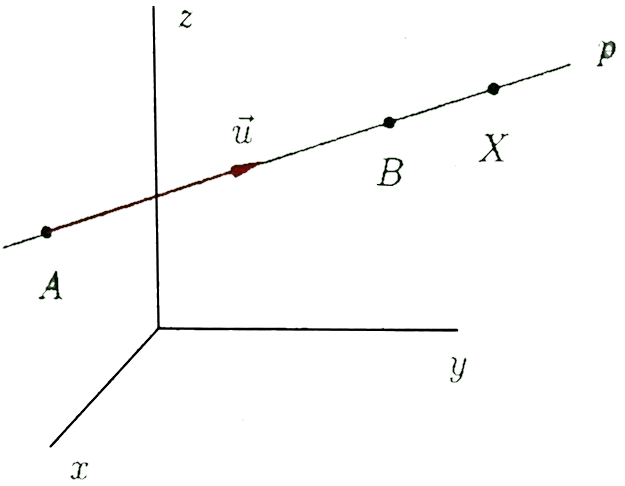
\includegraphics[width=0.4\linewidth]{mai_fig000.png}
    \captionof{figure}{Zadáni přímky. \cite[s.~1]{Musilova2009MA1}
    \label{mai:fig000}}
    \par}
  Veličinou \(t\), takzvaným \emph{parametrem}, který může nabývat všech reálných hodnot, 
  \(t\in\mathbb{R}\), dokážeme popsat všechny vektory \(\overrightarrow{AX}\), jejichž 
  koncový bod \(X\) leží na přímce \(p\). Naopak, žádné jiné body \(X\) než ty, které leží na 
  přímce \(p\), tuto vlastnost nemají. S označením bodů \(A\), \(X\), resp. vektorů 
  \(\vec{u}\), \(\overrightarrow{AX}\) kartézskými souřadnicemi, resp. složkami
  \begin{align*}
                    A &= (x_A,y_A, z_A), \\ 
                    X &=(x,y,z),         \\
              \vec{u} &= (u_1,u_2,u_3),  \\ 
  \overrightarrow{AX} &= (x - x_A, y - y_1A, z-z_A),
  \end{align*}
  dostáváme \textbf{parametrické vyjádřeni přímky} \(p\) ve tvaru
  \begin{equation}\label{MAI:eq_M001}
    p = \left\{(x,y,z)\in\mathbb{R}^3\,|\,
    \begin{matrix}
      x = x_A + tu_1,        \\
      y = y_A + tu_2,        \\
     z = z_A + tu_3,
    \end{matrix}
    \;t\in\mathbb{R}
    \right\}. 
  \end{equation}
  \normalsize
\end{example}
    %---------------------------------------------------------------
    
    Vidíme, že kartézské souřadnice bodu na přímce se vůči souřadnicím bodu \(A\) mění přímo 
    úměrně v závislosti na hodnotě parametru \(t\), tj. závisí na jeho první mocnině. Příslušná 
    závislost se nazývá \textbf{lineární funkcí}.
    
    Obdobně zapíšeme parametrické vyjádření roviny v \(\mathbb{R}^3\):
    
    %---------------------------------------------------------------
    % !TeX spellcheck = cs_CZ
\begin{mathexam}{Parametrická vyjádření roviny}{exam004}
  Rovina v trojrozměrném prostoru \(\mathbb{R}^3\) je zadána třemi body \(A\), \(B\) a \(C\), které
  nesmějí ležet v jedné přímce, popřípadě dvěma body \(A\) a \(B\) a vektorem \(\vec{v}\)
  nerovnoběžným s \(\overrightarrow{AB}\), anebo bodem \(A\) a dvěma nerovnoběžnými směrovými
  vektory \(\vec{u}\) a \(\vec{v}\) (obr. \ref{mai:FIG002}). Všechny tyto typy zadání jsou
  ekvivalentní. Lze volit například \(\vec{u} = \overrightarrow{AB}\), \(\vec{v} =
  \overrightarrow{AC}\). Je-li \(X\) libovolným bodem roviny \(\varrho\), jsou vektory
  \(\overrightarrow{AX}\), \(\vec{u}\) a \(\vec{v}\) \textbf{lineárně závislé}. To znamená, že
  existují taková reálná čísla \(r\) a \(s\), že vektor \(\overrightarrow{AX}\) lze zapsat jako
  lineární kombinaci

  \begin{equation*}
    \overrightarrow{AX} = r\cdot\vec{u} + s\cdot\vec{v}, \qquad r,s \in\mathbb{R}
  \end{equation*}
  Při obdobném zápisu kartézských souřadnic bodů a složek vektorů jako u vyjádření přímky dostaneme
  parametrické vyjádření roviny \(\varrho\)
  \begin{equation*}
    \varrho = \left\{
    \begin{matrix}  
      (x,y,z)\in\mathbb{R}^3  \\
      r, s \in\mathbb{R}
    \end{matrix}
    \,\left\lvert\,
    \begin{matrix}
      x = x_A + ru_1 + sv_1,        \\
      y = y_A + ru_2 + sv_2,        \\
      z = z_A + ru_3 + sv_3,
    \end{matrix}\right.          
    \right\}.
  \end{equation*} 

  { \centering
    \captionsetup{type=figure}
    \luafigure[1]{mai_fig026.pdf}
    \captionof{figure}{Zadání roviny. \cite[s.~3]{Musilova2009MA1}
    \label{mai:FIG002}} \par}

  Toto vyjádření obsahuje opět lineární závislost: Souřadnice \(x\), \(y\) a \(z\) se vůči
  souřadnicím bodu \(A\) mění v závislosti na prvních mocninách parametrů \(r\) a \(s\). Můžeme tak
  hovořit o jakési „vícerozměrné úměře“.
\end{mathexam}
  
    %---------------------------------------------------------------
    
    Všimněme si nyní příkladů linearity z oblasti přírodovědy.
    
    %---------------------------------------------------------------
    % !TeX spellcheck = cs_CZ
% \wikitextrule
\begin{mdframed}[style=mdexam]
  \begin{example}\label{mai:exam035}
    \textbf{Fyzika - Ohmův zákon:}\newline
    Z elektřiny víme, že některé vodiče či elektrické prvky se při průchodu elektrického proudu 
    chovají podle zákona linearity: Proud, který jimi protéká, závisí přímo úměrně na přiloženém 
    napětí (obr. \ref{mai:fig036}). Platí \(I(U) = R^{-1 }U\) s konstantou úměrnosti \(R^{-1}\), kde 
    \(R\) je elektrický odpor vodiče (prvku).

    Pozn. 1: Předpokládáme, že elektrický odpor voltmetru je tak velký, že proud jím procházející je 
    z hlediska přesnosti měření zanedbatelný.
    
    Pozn. 2: Graf závislosti proudu na napětí na obrázku \ref{mai:fig036} může pro vyšší hodnoty 
    napětí vykazovat odchylku od linearity (přímkové závislosti), neboť se prvek při vyšším proudu 
    zahřívá a jeho odpor roste.
    
    {\centering
      \captionsetup{type=figure}
      \luafigure[1]{mai_fig036.png}
      \captionof{figure}{Chování lineárního vodiče (Ohmův zákon). \cite[s.~15]{Musilova2009MA1}
      \label{mai:fig036}}
      \par}  
  \end{example}
\end{mdframed}
    %---------------------------------------------------------------

    %---------------------------------------------------------------
    % !TeX spellcheck = cs_CZ
\wikitextrule
\begin{example}\label{mai:exam036}
  \textbf{Fyzika — speciální typy pohybů:}\newline\small
  Při rovnoměrném pohybu tělesa (ať již přímočarém či křivočarém) je dráha, kterou těleso urazí za 
  dobu \(t\), přímo úměrná velikosti jeho rychlosti \(v\), tj. \(s(t) = s_0 + vt\). Při pohybu 
  rovnoměrně zrychleném (zpožděném) je lineární závislost velikosti rychlosti na čase, tj. \(v(t) = 
  v_0 \pm at\) při pohybu přímočarém (\(a\) je velikost zrychlení), nebo \(v(t) = v_0 \pm a_\tau 
  t\) při pohybu křivočarém (\(a_\tau\) je velikost průmětu zrychlení do směru tečny k 
  trajektorii tělesa — tečného zrychlení).
  \normalsize
\end{example}
    %---------------------------------------------------------------
    
  \subsection{Soustavy lineárních rovnic a jejich rychlé řešení}
    Příkladů linearity v přírodě bychom mohli nalézt bezpočet. Vraťme se však k matematice a k 
    problematice uvedené v názvu tohoto odstavce, k soustavám lineárních rovnic. Začněme 
    jednoduchou slovní úlohou ze základní školy:
    
    %---------------------------------------------------------------
    % !TeX spellcheck = cs_CZ
% \wikitextrule
\begin{mdframed}[style=mdexam]
  \begin{example}\label{mai:exam037}
    \textbf{Jeníček a Mařenka kradli ježibabě perník:}\newline
    Dohromady snědli \num{11} perníkových srdíček. Jeníček jich přitom zkonzumoval o \num{3} více
    než Mařenka. Otázka je tradiční - kolik srdíček snědl každý z nich? Označíme-li \(M\) počet
    kousků, které snědla Mařenka a \(J\) počet srdíček, na nichž si pochutnal Jenda, můžeme
    informace zadané v úloze zapsat takto:
    \begin{equation*}
      M + J = 11, \qquad J = M + 3.
    \end{equation*}
    
    Řešení není problémem, snadno vidíme, že \(M = 4\) a \(J = 7\).
  \end{example}
\end{mdframed}
    %---------------------------------------------------------------
    
    O samotné řešení této jednoduché úlohy v tuto chvíli nejde. Pojmenujme si však vztahy, které 
    jsme pro neznámé hodnoty \(M\) a \(J\) ze zadání úlohy dostali. Neznámé vystupují v 
    rovnicích v první mocnině, tedy \emph{lineárně}. Máme \emph{soustavu dvou rovnic} o dvou 
    neznámých \(M\) a \(J\). Úvahu snadno zobecníme: Předpokládejme, že máme neznámé veličiny
    \begin{equation*}
      (x_1, x_2, \ldots, x_n)
    \end{equation*}
    a máme o nich \(m\) informací, které lze zapsat ve tvaru lineárních rovnic (neznámé budou v 
    těchto rovnicích vystupovat v první mocnině),
    \begin{align}
      a_{11}x_1 + a_{12}x_2 + \ldots + a_{1n}x_n &= b_1,     \nonumber           \\
      a_{21}x_1 + a_{22}x_2 + \ldots + a_{2n}x_n &= b_2,     \label{mai:eq002}   \\
      .......................................... &= \ldots   \nonumber           \\
      a_{m1}x_1 + a_{m2}x_2 + \ldots + a_{mn}x_n &= b_m,     \nonumber
    \end{align}
    Soustavu (\ref{mai:eq002}) nazýváme soustavou \(m\) lineárních rovnic o \(n\) neznámých. 
    Označme ji jako \(S\) a pod tímto označením se k ní budeme vracet. Soubory reálných čísel 
    \((a_{ij})\) a \((b_i)\), kde \(1 < i < m\), \(1 \leq j < n\), jsou zadány. Lze je uspořádat 
    do takzvaných \textbf{matic}:
    \begin{equation}\label{mai:eq003}
      \matr{A} =
        \begin{pmatrix}
          a_{11} & a_{12} & \ldots & a_{1n} \\
          a_{21} & a_{22} & \ldots & a_{2n} \\
          \ldots & \ldots & \ldots & \ldots \\
          a_{m1} & a_{m2} & \ldots & a_{mn}          
        \end{pmatrix},
        \overline{\matr{B}} =
        \begin{pmatrix}
          b_1     \\
          b_2     \\
          \ldots  \\
          b_m 
        \end{pmatrix}
    \end{equation}
    
    Matice \(\matr{A}\) je typu \(m/n\), má \(m\) řádků a \(n\) sloupců, \(i\) je řádkový index a 
    \(j\) je sloupcový index. Matice \(\overline{\matr{B}}\) je typu \(m/1\) (\(m\) řádků a jeden 
    sloupec), hovoříme také o sloupcové matici. Soustavu \(S\) můžeme zapsat zkráceně pomocí 
    maticového násobení (podrobněji viz později odstavec \ref{mai:IchapIIsecIII}):
    \begin{equation*}
      \matr{A} \cdot \matr{X} = \matr{B}, \qquad \text{nebo}
    \end{equation*}  
    \begin{equation}\label{mai:eq004}
        \begin{pmatrix}
          a_{11} & a_{12} & \ldots & a_{1n} \\
          a_{21} & a_{22} & \ldots & a_{2n} \\
          \ldots & \ldots & \ldots & \ldots \\
          a_{m1} & a_{m2} & \ldots & a_{mn}
        \end{pmatrix}
        \cdot
        \begin{pmatrix}
          x_1     \\
          x_2     \\
          \ldots  \\
          x_m 
       \end{pmatrix}
        =
       \begin{pmatrix}
            b_1     \\
            b_2     \\
            \ldots  \\
            b_m 
          \end{pmatrix}
    \end{equation}
    V tuto chvíli vysvětlíme podstatu maticového násobení jen technicky: Násobit mezi sebou  můžeme matici 
    \(\matr{A} = (a_{ij})\) typu \(m/n\) (levý činitel) a matici \(\matr{A} = (c_{jk})\) typu 
    \(n/p\) (pravý činitel, činitele nelze zaměňovat). Výsledkem je matice \(\matr{A} = (d_{ik})\) 
    typu \(m/p\), jejíž prvky se počítají podle předpisu
    \begin{equation}\label{mai:eq005}
      d_{ik} = \sum_{j=1}^{n} a_{ij}\cdot c_{jk}.
    \end{equation}
    
    Z tohoto obecného předpisu vidíme, že levé strany soustavy \(S\) lze interpretovat ve tvaru 
    součinu matice \(A\) typu \(m/n\) s maticí neznámých typu \((n/1)\), výsledkem je matice 
    pravých stran \(\overline{\matr{B}}\), která je typu \(m/1\). Matice \(\matr{A}\) se nazývá 
    \textbf{maticí soustavy}. Matice, která vznikne jejím \emph{rozšířením} o sloupec pravých 
    stran, tj.
    \begin{equation}\label{mai:eq006}
      \matr{B} = (\matr{A}|\overline{\matr{B}}) =
      \left(
        \begin{array}{cccc|c}
          a_{11} & a_{12} & \ldots & a_{1n} & b_1    \\
          a_{21} & a_{22} & \ldots & a_{2n} & b_2    \\
          \ldots & \ldots & \ldots & \ldots & \ldots \\
          a_{m1} & a_{m2} & \ldots & a_{mn} & b_m
        \end{array}
      \right)
    \end{equation}
    je pak \textbf{rozšířenou maticí soustavy}. Je-li sloupec pravých stran soustavy tvořen 
    samými nulami, nazývá se soustava \textbf{homogenní}, v opačném případě \textbf{nehomogenní}. 
    Řešením soustavy \(S\) nazýváme každou \(n\)-tici \((x_i, x_2,\ldots, x_n)\), která soustavu 
    \(S\) splňuje. Cílem je najít všechna řešení soustavy \(S\). Abychom řešení nalezli, musíme 
    soustavu upravovat, zjednodušovat. Prováděné úpravy mají vést k jednodušší, avšak 
    ekvivalentní soustavě rovnic, tj. takové, která má naprosto stejný soubor všech řešení jako 
    soustava původní. Takové úpravy nazýváme \textbf{ekvivalentními}. Dvě základní, pomocí nichž 
    lze uskutečnit všechny ostatní, jsou
    \begin{itemize}\addtolength{\itemsep}{-0.5\baselineskip}
      \item vynásobení libovolné, například \(i\)-té, rovnice libovolným \emph{nenulovým} číslem,
      \item přičtení \(i\)-té rovnice vynásobené libovolným číslem k \(l\)-té rovnici.
    \end{itemize} 
    V soustavě lze samozřejmě také měnit pořadí rovnic. Tato úprava je rovněž ekvivalentní. 
    Nevypisujeme ji však zvlášť proto, že ji lze realizovat pomocí vhodně zvolené posloupnosti 
    základních dvou úprav.
    
    Abychom nemuseli soustavu stále opisovat i s neznámými, provádíme obvykle ekvivalentní 
    úpravy jen s maticí \(\matr{B} = (\matr{A}|\overline{\matr{B}})\) (každý řádek této matice 
    představuje jednu rovnici soustavy \(S\)). Může se stát, že soustava má právě \emph{jedno 
    řešení}, jako tomu bylo v  úloze o Mařence a Jeníčkovi. Také nemusí mít \emph{řešení žádné}, 
    jako například soustava \(x + y = 0\), \(x + y = 1\) (součet dvou čísel nemůže nabývat současně 
    dvou různých hodnot). A třeba má také řešení \emph{nekonečně mnoho} (řešením soustavy jedné 
    rovnice o dvou neznámých \(x + y = 1\) jsou všechny dvojice tvaru \((x, 1 - x)\), kde \(x\) je 
    libovolné). A může mít soustava \(S\) třeba právě dvě řešení? Prostřednictvím následujícího 
    příkladu ukážeme metodu, která vede velmi rychle k nalezení všech řešení a umožňuje také 
    vyslovit obecné závěry o jejich vlastnostech a počtu. Jedná se o \textbf{Gaussovu eliminační 
    metodu}.

    %---------------------------------------------------------------
    \begin{mathexam}{Gaussova eliminační metoda}{exam038}
  Je zadána soustava tří (\(m = 3\)) rovnic o pěti (\(n = 5\)) neznámých:
  \begin{alignat*}{7}
       x_1 &+ 2x_2 &-  x_3 &+  x_4 &- 5x_5 &=  &&0, \\
     -2x_1 &- 4x_2 &+ 2x_3 &+ 4x_4 &+ 4x_5 &= -&&6, \\
      -x_1 &- 2x_2 &+  x_3 &+ 5x_4 &-  x_5 &=  &&6.
  \end{alignat*}
  Budeme provádět ekvivalentní úpravy matice \(\matr{B}\) tak, abychom ji zjednodušovali.
  Ekvivalenci matic budeme označovat znakem \(\sim\). 
  \begingroup
    \renewcommand\arraystretch{1.0}
    \renewcommand\arraycolsep{3pt}
    \begin{equation*}
      \matr{B} = (\matr{A}\lvert\overline{\matr{B}}) =
      \left(
        \begin{array}{rrrrr|r}
           1 &  2 & -1 & 1 & -5 &  0    \\
          -2 & -4 &  2 & 4 &  4 & -6    \\
          -1 & -2 &  1 & 5 & -1 &  6
        \end{array}
      \right).
    \end{equation*}
  \endgroup
  V prvním řádku je na první pozici jednička. Toho využijeme k snadné „likvidaci“, tedy eliminaci,
  prvních prvků v druhém a třetím řádku pomocí elementárních úprav. Provedeme tyto dvě úpravy:
  první řádek vynásobený číslem \num{2} přičteme k druhému řádku, první řádek přičteme ke třetímu
  řádku. Dostaneme
  \begingroup
    \renewcommand\arraystretch{1.0}
    \renewcommand\arraycolsep{3pt}
    \begin{equation*}
      \matr{B} \sim
      \left(
        \begin{array}{rrrrr|r}
          1 &  2 & -1 & 1 & -5 &  0         \\
          \bm{0} &  0 &  0 & 6 & -6 & -6    \\
          \bm{0} &  0 &  0 & 6 & -6 &  6
        \end{array}
      \right).
    \end{equation*}
  \endgroup  
  Vidíme, že jsme v druhém i třetím řádku dostali na první sloupcové pozici nulu (tučná). (Nuly na
  dalších  pozicích vznikly náhodou, vlivem jednoduchosti zadání.) Nyní vynásobíme druhý i třetí
  řádek číslem (\num{1/6}):
  \begingroup
    \renewcommand\arraystretch{1.0}
    \renewcommand\arraycolsep{3pt}    
    \begin{equation*}
      \matr{B} \sim
      \left(
        \begin{array}{rrrrr|r}
                1 &  2 & -1 & 1 & -5 &  0    \\
                0 &  0 &  0 & 1 & -1 & -1    \\
                0 &  0 &  0 & 1 & -1 &  1
        \end{array}
      \right).
    \end{equation*}
  \endgroup  
  Přestože již nyní vidíme, že soustava nemá řešení (rovnice druhého a třetího řádku znějí \(x_4 -
  x_5 = - 1\) a \(x_4 -x_5 = 1\), takže jim nevyhovuje žádná dvojice čísel \((x_4, x_5)\)), budeme
  v eliminaci pokračovat. Další úpravy se již týkají pouze druhého a třetího řádku. Druhý řádek
  vynásobený (\num{-1}) přičteme ke třetímu. Pak

  \begingroup
  \renewcommand\arraystretch{1.0}
  \renewcommand\arraycolsep{3pt}
    \begin{equation*}
      \matr{B} \sim
      \left(
        \begin{array}{rrrrr|r}
                1 &  2 & -1 & 1      & -5 &  0    \\
                0 &  0 &  0 & 1      & -1 & -1    \\
                0 &  0 &  0 & \bm{0} &  0 &  2
        \end{array}
      \right).
    \end{equation*}
  \endgroup  
  Získáváme tak ekvivalentní soustavu rovnic
  \begin{alignat*}{5}
        x_1 + 2x_2 - x_3 &+  x_4 &- 5x_5 &=  &&0, \\
                         &+  x_4 &-  x_5 &= -&&1, \\
                         &       &     0 &=  &&2.
  \end{alignat*}
  V poslední rovnici je ihned vidět rozpor - soustava nemá řešení
\end{mathexam}
    %---------------------------------------------------------------

    Na základě výsledného tvaru matice soustavy a rozšířené matice soustavy získané ekvivalentními 
    úpravami soustavy \(S\) nyní formulujeme obecné kritérium pro to, aby soustava S měla
    vůbec nějaké řešení. Matice \(\matr{A}\) i \(\matr{B}\) se po provedení ekvivalentních úprav 
    dostaly do velmi jednoduchého tvaru, který připomíná schodiště obrácené „vzhůru nohama“, 
    odmyslíme-li si nuly v levé části jednotlivých řádků (následující zápis pouze usnadňuje 
    názornou představu, znak ekvivalence již psát nemůžeme):
    \begin{equation*}
      \matr{A} \ldots
      \left(
        \begin{array}{rrrrr}
                1 &  2 & -1 & 1      & -5     \\
                  &    &    & 1      & -1     \\
 
        \end{array}
      \right),
      \qquad
      \matr{B} \ldots
      \left(
        \begin{array}{rrrrr|r}
                1 &  2 & -1 & 1      & -5 &  0    \\
                  &    &    & 1      & -1 & -1    \\
        \end{array}
      \right).
    \end{equation*}
    
    Všimněme si, že „schodiště“ jsou nepravidelná, pokud jde o šířku schodů, výška všech schodů
    je však stejná - jeden řádek. Tímto způsobem je dán \emph{schodovitý tvar} matice \(\matr{A}\), 
    resp. \(\matr{B}\). Úzce s ním souvisí důležitá charakteristika matice, která je nezávislá jak 
    na provedených úpravách tak na výsledném schodovitém tvaru. Je to hodnost matice, definovaná 
    takto:
    
    \textbf{Hodnost} matice je počet nenulových řádků jejího schodovitého tvaru.
    
    V našem příkladu je hodnost matice \(A\) soustavy \(S\) rovna dvěma, hodnost matice rozšířené 
    \(\matr{B}\) je rovna třem. Píšeme
    \begin{equation*}
      h(\matr{A}) = 2,\qquad h(\matr{B}) = 3.
    \end{equation*}
    
    \begin{note}
      Lze získat schodovitý tvar různými posloupnostmi ekvivalentních úprav je zřejmé. Uvědomme si 
      však, že ani výsledný schodovitý tvar není určen jednoznačně - stačí třeba vynásobit některý 
      řádek dvěma a výsledná matice ekvivalentní s původní je rovněž schodovitá. Poněvadž má matice 
      \(\matr{B}\) o jeden sloupec více než matice \(\matr{A}\), platí vždy \(h(\matr{A}) < 
      h(\matr{B})\). V případě \(h(\matr{A}) < h(\matr{B})\) pak \(h(\matr{A}) = h(\matr{B}) - 1\). 
      Jak názorně ukazuje náš příklad, má pro \(h(\matr{A}) < h(\matr{B})\) některá z rovnic 
      ekvivalentní soustavy tvar \(0 = 1\), soustava tedy nemá řešení. Můžeme tak formulovat 
      kritérium (podmínku nutnou a postačující) řešitelnosti soustavy lineárních rovnic.
    \end{note}
    
    \begin{lemma}\label{mai:lemma001}
      (\textbf{Frobeniova}): Soustava lineárních rovnic má řešení právě tehdy, je-li hodnost její 
      matice rovna hodnosti matice rozšířené.
    \end{lemma}
    
    Ihned vidíme, že homogenní soustava má podle této věty řešení vždy, neboť poslední sloupec její 
    rozšířené matice je složen ze samých nul. Skutečně, jedním ze souboru řešení každé
    homogenní soustavy je \(n\)-tice
    \begin{equation*}
      (x_1, x_2, \ldots, x_n) = (0, 0, \ldots, 0),
    \end{equation*}
    zvaná \textbf{triviální řešení}.
    
    Nyní se vraťme k otázce, jak zjistit, kolik řešení má daná soustava, a jak je všechna popsat.
    Poslouží nám příklad \ref{mai:exam038} v mírné obměně spočívající v záměně koeficientu \(b_3\) 
    z hodnoty \num{6} na \num{-6}.
    
    %---------------------------------------------------------------
    % !TeX spellcheck = cs_CZ
\wikitextrule
\begin{example}\label{mai:exam039}
  \textbf{Ještě jednou Gaussova eliminační metoda}\newline\small
  Je zadána soustava rovnic:
  \begin{alignat*}{7}
      x_1 &+ 2x_2 &-  x_3 &+  x_4 &- 5x_5 &=  &&0, \\
    -2x_1 &- 4x_2 &+ 2x_3 &+ 4x_4 &+ 4x_5 &= -&&6, \\
     -x_1 &- 2x_2 &+  x_3 &+ 5x_4 &-  x_5 &= -&&6.
  \end{alignat*}
  Rozšířená matice soustavy má nyní tvar 
  \begin{equation*}
    \matr{B} = (\matr{A}|\overline{\matr{B}}) =
    \left(
      \begin{array}{rrrrr|r}
         1 &  2 & -1 & 1 & -5 &  0    \\
        -2 & -4 &  2 & 4 &  4 & -6    \\
        -1 & -2 &  1 & 5 & -1 & -6
      \end{array}
    \right).
  \end{equation*}
  Stejné ekvivalentní úpravy jako v příkladu \ref{mai:exam038} vedou nyní k výsledku
  \footnotesize %\small \scriptsize \tiny
  \begin{equation*}
    \matr{B} \sim
    \left(
      \begin{array}{rrrrr|r}
         1 &  2 & -1 & 1 & -5 &  0         \\
         \bm{0} &  0 &  0 & 6 & -6 & -6    \\
         \bm{0} &  0 &  0 & 6 & -6 & -6
      \end{array}
    \right) \sim
    \left(
      \begin{array}{rrrrr|r}
              1 &  2 & -1 & 1 & -5 &  0    \\
              0 &  0 &  0 & 1 & -1 & -1    \\
              0 &  0 &  0 & 1 & -1 & -1
      \end{array}
    \right) \sim
    \left(
      \begin{array}{rrrrr|r}
              1 &  2 & -1 & 1      & -5 &  0    \\
              0 &  0 &  0 & 1      & -1 & -1    \\
              0 &  0 &  0 & \bm{0} &  0 &  0
      \end{array}
    \right).
  \end{equation*}\normalsize
  Nyní platí \(h(\matr{A}) = h(\matr{B}) = 2\). Podle Frobeniovy věty \ref{mai:lemma001} tedy 
  soustava určitě má řešení. Ekvivalentní soustava má tvar
  \begin{alignat*}{5}
         x_1 + 2x_2 - x_3 &+  x_4 &- 5x_5 &=  &&0, \\
                          &+  x_4 &-  x_5 &= -&&1, \\
                          &       &     0 &=  &&0.
  \end{alignat*}
  Poslední rovnice je identitou a můžeme ji vypustit. Máme pět neznámých a jen dvě nezávislé 
  rovnice. Dvě z neznámých tedy můžeme vyjádřit pomocí zbývajících. Postupujeme „odzadu“ , začínáme 
  druhou, jednodušší, rovnicí:
  \begin{align*}
                                                x_4 &= -1 + x_5,                \\
    x_1 = - 2x_2 + x_3 - x_4 + 5x_5 \Rightarrow x_1 &= -2x_2 + x_3 + 4x_5 + 1.
  \end{align*}
  Za neznámé vystupující na pravé straně, tj. \(x_2\), \(x_3\) a \(x_5\), můžeme dosazovat cokoli a 
  vždycky se k nějakým hodnotám \(x_1\) a \(x_4\) dopočítáme. Všechna řešení soustavy \(S\) proto 
  můžeme zapsat v obecném tvaru
  \begin{equation}\label{mai:eq040}
    (-2x_2 + x_3 + 4x_5 + 1, x_2, x_3, x_5 - 1, x_5).
  \end{equation}
  \normalsize
\end{example}
    %---------------------------------------------------------------
    
    Soubor řešení ve tvaru (\ref{mai:eq040}) se nazývá obecným řešením soustavy. Jeho jednotlivé 
    prvky, jednotlivá konkrétní řešení soustavy, jsou dány volbou volných neznámých \(x_2\), 
    \(x_3\) a \(x_5\). Také z příkladu \ref{mai:exam039} lze učinit obecný závěr:
    
    \begin{lemma}\label{mai:lemma002}
      Nechť pro soustavu \(m\) lineárních rovnic o \(n\) neznámých platí \(h(\matr{A}) = 
      h(\matr{B}) = h\). Pak její obecné řešení závisí (lineárně) na \(d = n - h\) volných 
      neznámých.
    \end{lemma}
    
    Číslo \(d\) se nazývá \textbf{dimenze prostoru řešení soustavy}. Tento pojem ještě podrobněji 
    vysvětlíme později.
    
    Nyní již snadno zodpovíme otázku, čím je dána mohutnost souboru řešení soustavy lineárních 
    rovnic, tj. kolik má taková soustava řešení. Možnosti jsou pouze:
    \begin{itemize}
      \item žádné řešení - pro \(h(\matr{A}) \neq h(\matr{B})\),
      \item právě jedno řešení - pro \(h = h(\matr{A}) = h(\matr{B})\) a současně \(h = n\), takže 
            nezbývá žádná volná neznámá,
      \item nekonečně mnoho řešení - pro \(h = h(\matr{A}) = h(\matr{B})\) a současně \(h < n\),  
            kdy máme k dispozici \(d = n - h\) volných neznámých.
    \end{itemize}    
    Že by tedy třeba měla soustava právě dvě, tři či osmnáct řešení není možné.
    
    Jakési zvláštní postavení můžeme přisoudit homogenním soustavám. Ty mají, jak jsme se
    již přesvědčili, řešení vždy, alespoň to triviální, složené ze samých nul. Zajímejme se o 
    situaci, kdy má homogenní soustava i jiná, netriviální, řešení. U homogenní soustavy je 
    hodnost její matice vždy shodná s hodností matice rozšířené, \(h = h(\matr{A}) = h(\matr{B})\). 
    Je-li navíc \(h = n\), má podle obecného tvrzení \ref{mai:lemma002} soustava právě jedno 
    řešení, jímž nutně je řešení triviální. V opačném případě, tj. pro \(h < n\), máme opět k 
    dispozici \(d = n - h\) volných neznámých, a tedy nekonečně mnoho netriviálních řešení. 
    Všimněme si ještě jedné zajímavosti u homogenní soustavy. Jsou-li dvě \(n\)-tice čísel \(X = 
    (x_1, x_2, \ldots, x_n)\) a \(\overline{X} = (\overline{x}_1, \overline{x}_2, \ldots, 
    \overline{x}_n)\) jejím řešením, pak také \(n\)-tice vytvořená jako jejich lineární kombinace
    \begin{equation*}
      \alpha\cdot X + \overline{\alpha}\cdot\overline{X} = 
        (\alpha x_1, \alpha x_2, \ldots, \alpha x_n) + 
        (\overline{\alpha}\,\overline{x}_1, 
        \overline{\alpha}\,\overline{x}_2, \ldots, 
        \overline{\alpha}\,\overline{x}_n)
    \end{equation*}
    kde \(\alpha\) a \(\overline{\alpha}\) jsou libovolná čísla, je \emph{řešením soustavy}. 
    Možnost tohoto „lineárního kombinování“ připadá samozřejmě v úvahu pro libovolný počet 
    libovolných řešení soustavy. Fyzik by řekl, že soustava vyhovuje principu superpozice. 
    Soustava nehomogenní tu to vlastnost nemá „vinou“ nenulového sloupce 
    pravých stran.
    
    \subsection{Přímky a roviny - lineární geometrické útvary}
      Vraťme se ještě na chvíli k linearitě v geometrii a všimněme si problematiky vzájemné polohy
      přímek a rovin. Procvičíme si na ní mimo jiné i řešení soustav lineárních rovnic. V odstavci 
      \ref{mai:IchapIIsecI} jsme odvodili parametrické vyjádření přímky a roviny v trojrozměrném 
      prostoru. Nyní se pokusíme z těchto vyjádření vyloučit parametry a získat obecné rovnice 
      přímky a roviny, které již budou obsahovat pouze kartézské souřadnice bodů ležících v 
      příslušné přímce či rovině. Začněme případem roviny.

      %---------------------------------------------------------------
      % !TeX spellcheck = cs_CZ
\wikitextrule
\begin{example}\label{mai:exam040}
  \textbf{Obecná rovnice roviny}\newline\small
  Parametrické rovnice roviny z příkladu \ref{mai:exam004} můžeme chápat jako soustavu tří rovnic o 
  dvou neznámých:
  \begin{align*}
      ru_1 + sv_1 &= x - x_A, \\
      ru_2 + sv_2 &= y - y_A, \\
      ru_3 + sv_3 &= z - z_A, 
  \end{align*}
  kde neznámými jsou parametry \(r\) a \(s\). Z geometrického významu této soustavy je zřejmé, že 
  pro každý bod \(X = (x, y, z)\), který leží v rovině \(\varrho\), bude soustava mít jako řešení 
  právě jednu dvojici parametrů \((r, s)\) (pro body, které v rovině neleží, soustava řešení nemá). 
  Vypočteme parametry \(r\) a \(s\) například z prvních dvou rovnic. Předpokládejme, že \(u_1 \neq 
  0\), a upravujme matici soustavy:
  
  \begin{equation*}
    \left(
      \begin{array}{rr|r}
         u_1 &  v_1  &  x-x_A         \\
         u_2 &  v_2  &  y-y_A
      \end{array}
    \right) \sim
    \left(
      \begin{array}{cc|c}
              u_1 &  v_1               & x - x_A     \\
              0   &  u_1v_2 - u_2v_1   & (y-y_A)u_1 - (x-x_A)u_2
      \end{array}
    \right).
  \end{equation*}
  odkud pro \((u_1v_2 — u_2v_1) \neq 0\) dostaneme
  \begin{equation*}
    r = - \dfrac{(y-y_A)v_1 - (x-x_A)v_2}{u_1v_2 - u_2v_1}, \qquad 
    s =   \dfrac{(y-y_A)u_1 - (x-x_A)u_2}{u_1v_2 - u_2v_1}
  \end{equation*}
  Dosadíme-li získané hodnoty do třetí rovnice (dá to trochu práce), dostáváme obecnou  rovnici roviny 
  \(\varrho\)
  \begin{subequations} % \label{mai:eq041}
    \begin{equation}\label{mai:eq041a}
      ax + by + cz + d= 0,
    \end{equation}
    \begin{equation}\label{mai:eq04b}
      a = u_2v_3 - u_3v_2, \qquad b = u_3v_1 - u_1v_3, \qquad c = u_1v_2 - u_2v_1,
    \end{equation}
    \begin{equation}\label{mai:eq041c}
      d = (u_2v_3 - u_3v_2)x_A - (u_3v_1 - u_1v_3)y_A - (u_1v_2 - u_2v_1)z_A.
    \end{equation}
  \end{subequations}
  Při tomto výpočtu vyvstaly některé problémy. Pokusme se je vyřešit:
  \begin{itemize}
    \item Aby získaná rovnice opravdu představovala nějakou rovinu, musí v ní zůstat alespoň jedna 
          ze souřadnic \(x, y, z\). Alespoň jedno z čísel \(a, b, c\) by tedy mělo být nenulové. 
          Dokažte, že tomu tak opravdu je, a využijte při tom skutečnosti, že vektory \(\vec{u}\) a 
          \(\vec{v}\) nesmí být rovnoběžné. Co znamená předpoklad \((u_1v_2 - u_2v_1) \neq 0\)?
    \item Předpokládali jsme, že \(u_1 \neq 0\). Jak budeme postupovat, nebude-li tento předpoklad  
          splněn? Lze v tomto případě použít obecné výrazy získané pro \(r\) a \(s\)?
  \end{itemize}
  \normalsize
\end{example}
      %---------------------------------------------------------------

      %---------------------------------------------------------------
      % !TeX spellcheck = cs_CZ
% \wikitextrule
\begin{mdframed}[style=mdexam]
  \begin{example}\label{mai:exam041}
    \textbf{Obecná rovnice přímky}\newline
    Přímku \(p\) si snadno představíme jako průsečnici dvou nerovnoběžných rovin \(\varrho\) a 
    \(\sigma\). Jejich rovnice tvoří soustavu, která představuje obecné rovnice přímky
      \begin{align*}
        \varrho &= \{(x, y, z)\in\mathbb{R}^3\mid a_1x+ b_1y+ c_1z+ d_1 = 0 \}  \\ 
        \sigma  &= \{(x, y, z)\in\mathbb{R}^3\mid a_2x+ b_2y+ c_2z+ d_2 = 0 \}, 
      \end{align*}
    Zkusme přijít na to, co musí platit pro koeficienty v rovnicích rovin, aby byly nerovnoběžné. 
    Jedna a táž přímka může být zadána různými dvojicemi nerovnoběžných rovin. Všechny roviny, které 
    přímkou \(p\) procházejí, tvoří geometrický útvar zvaný \textbf{svazek rovin prvního druhu}, 
    přímka sama je \textbf{osou} svazku. 
  \end{example}
\end{mdframed}
      %---------------------------------------------------------------
      
      %---------------------------------------------------------------
      % !TeX spellcheck = cs_CZ
\wikitextrule
\begin{example}\label{mai:exam042}
  \textbf{Vektor rovnoběžný s rovinou}\newline\small
   Ja k poznáme, zda je vektor \(\vec{u} = (u_1, u_2, u_3)\) rovnoběžný s rovinou \(ax + by + cz + 
   d = 0\)? Pokud vektor \(\vec{u}\) s rovinou rovnoběžný je, pak zcela jistě existují v této 
   rovině dva body \(A = (x_A, y_A, z_A)\) a \(B = (x_B, y_B, z_B)\) tak, že \(\overrightarrow{AB} 
   = \vec{u} = (x_B - x_A, y_B - y_A, z_B - z_A)\). Tyto body splňují rovnici roviny, tj.
   \begin{equation*}
     ax_A + by_A + cz_A + d = 0,\qquad ax_B + by_B + cz_B + d = 0.
   \end{equation*}
   Odečtením rovnic dostaneme kritérium rovnoběžnosti vektoru s rovinou \(au_1 + bu_2+ cu_3 = 0\).
   \normalsize
\end{example}
      %---------------------------------------------------------------
  
      Máme připraveno vše pro řešení otázky vzájemné polohy přímek a rovin.

      %---------------------------------------------------------------
      % !TeX spellcheck = cs_CZ
\wikitextrule
\begin{example}\label{mai:exam043}
  \textbf{Vzájemná poloha tří rovin}\newline\small
  Zapojme geometrickou představivost a uvažujme, jakou vzájemnou polohu mohou mít tři roviny
  \begin{align*}
    \varrho: a_1x + b_1y + c_1z + d_1 &= 0, \\
    \sigma : a_2x + b_2y + c_2z + d_2 &= 0, \\
    \tau   : a_3x + b_3y + c_3z + d_3 &= 0,
  \end{align*}
  Současně si uvědomme, že předchozí soustava je soustavou lineárních rovnic o neznámých \(x\), 
  \(y\) a \(z\), představujících souřadnice společných bodů rovin \(\varrho\), \(\sigma\) a 
  \(\tau\). Soustava je charakterizována maticí
  \begin{equation}\label{mai:eq043}
    \matr{B} = (\matr{A}|\overline{\matr{B}}) =
    \left(
      \begin{array}{rrr|r}
         a_1 & b_1 & c_1 & -d_1    \\
         a_2 & b_2 & c_2 & -d_2    \\
         a_3 & b_3 & c_3 & -d_3
      \end{array}
    \right).
  \end{equation}
  Jsou tyto možnosti:
  \begin{itemize}
    \item Roviny mají společný právě jeden bod. V tomto případě musí mít soustava (\ref{mai:eq043}) 
          právě jedno řešení, a tedy \(h(\matr{A}) = h(\matr{B}) = 3\). (Útvar, který by vytvořily 
          všechny roviny procházející tímto bodem, se nazývá \textbf{trs rovin prvního druhu}, 
          společný bod je vrchol trsu.)
    \item Roviny mají společnou přímku. Řešení soustavy (\ref{mai:eq043}) bude v takovém případě 
          závislé na jedné volné neznámé (parametr bodů na společné přímce), takže \(h(\matr{A}) = 
          h(\matr{B}) = 2\). (Útvar, který by vytvořily všechny roviny procházející touto přímkou, 
          jsme před chvílí nazvali \textbf{svazkem rovin prvního druhu}, společná přímka je 
          \textbf{osou} svazku.)
    \item Roviny jsou totožné. Řešení soustavy (\ref{mai:eq043}) je popsáno dvěma volnými neznámými 
          (parametry bodů ve společné rovině), je tedy \(h(\matr{A}) = h(\matr{B}) = 1\).
    \item Roviny nemají společný žádný bod, mají však společný právě jeden směr (představme si 
          například nekonečně dlouhý stan „áčko“, v němž jedna z rovin tvoří podlážku a zbylé dvě 
          jsou stěnami). Společný směr \(\vec{u}\) je řešením homogenní soustavy rovnic (příklad 
          \ref{mai:exam043})
          \begin{align}\label{mai:eq044}
            a_1u_1 + b_1u_2+ c_1u_3 &= 0, \\
            a_2u_1 + b_2u_2+ c_2u_3 &= 0, \\
            a_3u_1 + b_3u_2+ c_3u_3 &= 0.
          \end{align}
           jejíž řešení musí být popsáno jednou volnou neznámou, tj. \(h(\matr{A}) = 2\). Původní 
           nehomogenní soustava (\ref{mai:eq043}) pro společné body rovin však řešení nemá, je tedy 
           \(h(\matr{B}) = 3\). (Útvar, který by vytvořily všechny roviny obsahující společný směr, 
           se nazývá \textbf{trs rovin druhého druhu}.)
    \item Roviny jsou rovnoběžné, nemají však žádný společný bod. Znamená to, že mají společné 
          dva nezávislé směry, řešení homogenní soustavy (\ref{mai:eq044}) obsahuje dvě volné 
          neznámé a platí \(h(\matr{A}) = 1\), \(h(\matr{B}) = 2\).
  \end{itemize}
  \normalsize
\end{example}
      %---------------------------------------------------------------

      %---------------------------------------------------------------
      % !TeX spellcheck = cs_CZ
\wikitextrule
\begin{example}\label{mai:exam044}
  \textbf{Vzájemná poloha dvou přímek}\newline\small
  Dvě přímky \(p\) a \(q\) jsou určeny dvěma dvojicemi rovin. Jejich společné body jsou tedy 
  řešením soustavy čtyř lineárních rovnic o třech neznámých (pišme rovnou rozšířenou matici 
  soustavy):
  \begin{equation}\label{mai:eq045}
    \matr{B} = (\matr{A}|\overline{\matr{B}}) =
    \left(
      \begin{array}{rrr|r}
         a_1 & b_1 & c_1 & -d_1    \\
         a_2 & b_2 & c_2 & -d_2    \\
         a_3 & b_3 & c_3 & -d_3    \\
         a_4 & b_4 & c_4 & -d_4
      \end{array}
    \right).
  \end{equation}
  Protože soustava obsahuje rovnice dvojic nerovnoběžných rovin, je \(h(\matr{A}) \geq 2\) 
  (zdůvodněte podrobněji). Možnosti vzájemné polohy přímek \(p\) (první dvě rovnice) a \(q\) (druhé 
  dvě rovnice) jsou tyto:
  \begin{itemize}
    \item Přímky jsou mimoběžné, nemají tedy žádný společný bod a roviny, které je určují, nemají 
          žádný společný směr. Soustava (\ref{mai:eq045}) nemá řešení, odpovídající homogenní 
          soustava pak rovněž ne, kromě řešení triviálního. Je tedy \(h(\matr{A}) = 3\), 
          \(h(\matr{B}) = 4\).
    \item Přímky jsou různoběžné, mají tedy společný právě jeden bod. Soustava (\ref{mai:eq045}) má 
          právě jedno řešení, a proto \(h(\matr{A}) = h(\matr{B}) = 3\).
    \item Přímky jsou rovnoběžné. Nemají tedy žádný společný bod, soustava nemá řešení, ale roviny, 
          které je určují, mají společný směr. To odpovídá situaci \(h(\matr{A}) = 23\), 
          \(h(\matr{B}) = 3\).
    \item Přímky jsou totožné. Řešení soustavy je popsáno jednou volnou neznámou, tj. \(h(\matr{A}) 
          = h(\matr{B}) = 2\)
  \end{itemize}
  \normalsize
\end{example}
      %---------------------------------------------------------------
      
      %---------------------------------------------------------------
      % !TeX spellcheck = cs_CZ
\wikitextrule
\begin{example}\label{mai:exam045}
  \textbf{Vzájemná poloha přímky a roviny}\newline\small
  Tuto úlohu převeďme na problém vzájemné polohy tří rovin a odpovězme si sami. Společně vyřešíme 
  konkrétní případ. Rozhodněme o vzájemné poloze přímky a roviny, najděme jejich společné body a 
  směry:
  \begin{align*}
    p       &: x + y + z + 5 = 0, \qquad 2x + 3y + 6z - 10 = 0 \\
    \varrho &: y + 4z + 17   = 0.
  \end{align*}
  \begin{equation*}
    \matr{B} = (\matr{A}|\overline{\matr{B}}) =
    \left(
      \begin{array}{rrr|r}
         1 & 1 & 1 & -5    \\
         2 & 3 & 6 &  10   \\
         0 & 1 & 4 & -17
      \end{array}
    \right)\sim
    \left(
      \begin{array}{rrr|r}
         1 & 1 & 1 & -5    \\
         0 & 1 & 4 &  20   \\
         0 & 1 & 4 & -17
      \end{array}
    \right)\sim
    \left(
      \begin{array}{rrr|r}
         1 & 1 & 1 & -5    \\
         0 & 1 & 4 &  20   \\
         0 & 0 & 0 & -37
      \end{array}
    \right).
  \end{equation*}
  Matice \(\matr{A}\) i \(\matr{B}\) jsme upravili do schodovitého tvaru. Vidíme, že \(h(\matr{A}) 
  = 2\), \(h(\matr{B}) = 3\). Soustava nemá řešení přímka \(p\) a rovina \(\varrho\) nemají žádný 
  společný bod. Jediná možnost, jak to zařídit, je, že přímka \(p\) je s rovinou \(\varrho\) 
  rovnoběžná. Mají společný směr, který je řešením homogenní soustavy o matici
  \begin{equation*}
    \matr{A} =
    \left(
      \begin{array}{ccc}
         1 & 1 & 1   \\
         2 & 3 & 6   \\
         0 & 1 & 4 
      \end{array}
    \right)\sim
    \left(
      \begin{array}{ccc}
         1 & 1 & 1   \\
         0 & 1 & 4   \\
         0 & 0 & 0 
      \end{array}
    \right).
  \end{equation*}
  Schodovitý tvar matice odpovídá ekvivalentní soustavě rovnic
  \begin{equation*}
    u_1 + u_2 + u_3 = 0,\qquad u_2 + 4u_3 = 0,
  \end{equation*}
  jejíž řešení je tvaru \((u_1, u_2, u_3) = (3u_3, -4u_3, u_3)\). Společný směr přímky \(p\) a 
  roviny \(\varrho\) je tedy určen například směrovým vektorem \((3, -4, 1)\) (pro \(u_3 = 1\)) 
  nebo kterýmkoli jeho nenulovým násobkem.
  \normalsize
\end{example}
      %---------------------------------------------------------------
      
%--------------------------------------------------------------------------------------------------
  \section{Počítání s čísly}\label{mai:IchapIIsecII}
    Někdo se jistě pozastaví nad tím, že jej chceme učit počítání s čísly. To přece každý umí
    už od základní školy! Jenže základní a do značné míry i střední škola nás učí počítat jen
    s určitým typem čísel - s čísly reálnými. Pravidla pro počítání s nimi se pro „běžné uživatele“
    stala natolik rutinní záležitostí, že už o nich vůbec nepřemýšlejí, nehledají v nich 
    zákonitosti, a kdybychom se jich zeptali, kde se tato pravidla vzala, pravděpodobně budou s 
    odpovědí velmi váhat. Pravidla pro jakékoli početní operace totiž skutečně nelze z ničeho 
    odvodit, ta je třeba definovat, samozřejmě tak, aby měla rozumné praktické vlastnosti.
    
    \subsection{Reálná čísla}
      U reálných čísel se opravdu dlouho nezdržíme, s těmi snad opravdu každý umí počítat. Všimneme 
      si jen trochu podrobněji struktury množiny všech reálných čísel, \textbf{reálné osy} 
      \(\mathbb{R}\). Zobrazit  reálná čísla na reálné ose, tedy na přímce, umíme proto, že na 
      množině reálných čísel je definováno \textbf{úplné uspořádání} „< “:
      \begin{itemize}
        \item Je-li současně \(a ≤ b\) a \(b ≤ a\), pak \(a = b\) 
              pro všechna \(a, b\in\mathbb{R}\ldots\) \textbf{antisymetrie},
        \item je-li současně\( a ≤ b\) a \(b ≤ c\), pak \(a ≤ c\) 
              pro všechna \(a,b,c\in\mathbb{R}\ldots\) \textbf{tranzitivita},
        \item \(a ≤ a\) pro všechna \(a\in\mathbb{R}\ldots\) \textbf{reflexivita},
        \item platí \(a ≤ b\) nebo \(b ≤ a\) pro všechna \(a, b \in\mathbb{R}\ldots\) 
              \textbf{úplnost}.
      \end{itemize}
      Pro každá dvě čísla \(a\) a \(b\) tedy dokážeme rozhodnout, zda jsou shodná (\(a = b\)), nebo 
      zda \(a\) je menší (\(a < b\)) či větší (\(a > b\)) než \(b\). Platí:
      \begin{itemize}
        \item Je-li současně \(a < b\) a \(c < d\), pak \(a + c < b + d\),
        \item je-li současně \(a < b\) a \(c > 0\), pak \(ac < bc\),
        \item je-li současně \(a < b\) a \(c < 0\), pak \(ac > bc\).
      \end{itemize}
      
      Množina reálných čísel obsahuje tyto důležité podmnožiny:
      \begin{itemize}
        \item Množinu přirozených čísel \(\mathbb{N} = \{1, 2, \ldots, n, \ldots\}\). Platí princip 
              \textbf{úplné indukce}: Je-li \(\mathbb{M} \subseteq \mathbb{N}\) nějaká množina 
              přirozených čísel, která obsahuje číslo \num{1} a která současně s každým číslem 
              \(n\) obsahuje i \(n + 1\), pak \(\mathbb{M} = \mathbb{N}\).
        \item Množinu celých čísel \(\mathbb{Z} = \{\ldots, -n, \ldots, -2, -1, 0, 1, 2, \ldots, m, 
              \ldots\}\).
        \item Množinu racionálních čísel \(\mathbb{Q}\) (zlomky). Racionální čísla lze vyjádřit 
              konečnými desetinnými zlomky (například \(p/q = 1/4 = \num{0.25}\)), nebo nekonečnými 
              periodickými desetinnými zlomky (například \(p/q = 4/3 = 1,33\ldots33\ldots = 
              1,\overline{3}\), \(p/q = 24/11 = 2,1818\ldots1818\ldots = 2,\overline{18}\)).
        \item Množinu iracionálních čísel, tj. čísel, která nejsou racionální. Iracionálními čísly 
              jsou neracionální řešení algebraických rovnic, například \(x^2 - 2 = 0 \Rightarrow x 
              = \sqrt{2}\), nebo \(x = - \sqrt{2}\) (čísla algebraická), a čísla typu \(\pi\), 
              \(e\), atd. (čísla transcendentní). Iracionální čísla jsou vyjádřena       
              nekonečnými neperiodickými desetinnými zlomky, např. 
              \(e = \num{2.718281828459545}\ldots\). Mezi každými dvěma reálnými čísly leží 
              nekonečně mnoho čísel racionálních i nekonečně mnoho čísel iracionálních.
      \end{itemize}
      
      Pro počítání s reálnými čísly jsou zavedeny základní operace, s nimiž umíme pracovat na
      základě zkušenosti, sčítání \(a + b\), odčítání \(a - b\), násobení \(a \cdot b\), resp. 
      \(ab\) a dělení \(a : b\). Ve skutečnosti jsou potřeba jen dvě, neboť odčítání je odvozeno 
      pomocí sčítání a dělení pomocí násobení. Uvědomili jste si někdy základní vlastnosti těchto 
      operací? Možná ne, ale pracujeme s nimi zcela samozřejmě:
%      \begin{table}[ht!]
%        \centering
%%        \begin{tabular}{l>{\centering}m{5cm}} %{@{}ll@{}}
%%\begin{tabular}{| c | >{\centering}m{5cm} |}
%%        \toprule
%%          \(a + b = b + a\)            & komutativní zákon pro součet  \\ %\midrule
%%          \((a + b) + c = a + (b +c)\) & asociativní zákon pro součet  \\
%%          \(a + 0 = 0 + a = a\)        & existence univerzálního neutrálního prvku \num{0}  \\
%%          \(a + (—a) = (—a) + a = 0\)  & existence právě jednoho opačného prvku k číslu \(a\)   \\ 
%%          \(ab = ba\)                  & komutativní zákon pro součin \\
%%          \(a(bc) — (ab)c\)            & asociativní zákon pro součin \\
%%          \(a(b + c) = ab + ac\)       & 1. distributivní zákon  \\
%%          \((b+ c)a — ba + ca\)        & 2. distributivní zákon \\
%%          \(a \cdot 1 = 1 \cdot a\)    & existence univerzálního jednotkového prvku 1 \\
%%          \(aa^{-1} = a^{-1}a\)        & existence právě jednoho inverzního prvku k číslu \(a\), pokud 
%%                                         \(a\neq 0\)\\
%%          \(ab = 0 \Leftrightarrow a = 0\) nebo \(b = 0\)) & neexistence dělitelů nuly \\
%%         \bottomrule
%%        \end{tabular}
%%\begin{tabular}{| c | >{\centering}m{5cm} |}
%% Bcd & A long cell with text that wraps around and is centered
%%\end{tabular}
%      \end{table}
      Odčítání a dělení:
      \begin{equation*}
        a — b = a + (—b), a:b = ab^{-1}, \qquad\text{pokud } b\neq0.
      \end{equation*}
      
    \subsection{Komplexní čísla}
      Komplexními čísly rozumíme uspořádané dvojice \([x, y]\) čísel reálných, pro které zavedeme 
      určité operace. Uspořádaností dvojice zde myslíme to, že jedno z čísel (v našem zápisu \(x\)) 
      je umístěno na první pozici dvojice a představuje reálnou část čísla \(z\), \(x = 
      \operatorname{Re}(z)\), druhé (v našem zápisu \(y\)) je na druhé pozici a je imaginární částí 
      čísla \(z\), \(y = \operatorname{Im}(z)\). Je tedy obecně  \( [x, y] ≠ [y, x]\). Množinu
    \subsection{Cvičení}
%--------------------------------------------------------------------------------------------------
  \section{Počítání s maticemi}\label{mai:IchapIIsecIII}
    \subsection{Základní operace s maticemi a hodnost matic}\label{mai:IchapIIsecIIIsubI}
    \subsection{Hodnost matic}\label{mai:IchapIIsecIIIsubII}
    \subsection{Násobení  matic}\label{mai:IchapIIsecIIIsubIII}
    \subsection{Čtvercová matice}\label{mai:IchapIIsecIIIsubIV}
    Algebra matic, tedy počítání s nimi, je v praxi zase jen počítání s čísly, samozřejmě podle
    specifických pravidel. S maticemi jsme se již setkali v odstavci \ref{mai:IchapIIsecI}, kde 
    jsme jich využili jako vhodné „pomůcky“ při řešení soustav rovnic. Nyní posuneme naše 
    znalosti o nich na poněkud vyšší úroveň. Zavedeme na množině matic \emph{algebraickou 
    strukturu}, která nám umožní s nimi počítat nezávisle na jejich vztahu k nějakým praktickým 
    aplikacím. Víme již, že maticí typu \(m/n\) (též obdélníková matice) rozumíme soubor reálných, 
    popřípadě i komplexních čísel uspořádaných do \(m\) řádků a \(n\) sloupců:
    
    \begin{definition}\label{def_matice}
      Nechť \(m, n\) jsou přirozená čísla. Jestliže každé uspořádané dvojici \((m,n)\in 
      \{1,2,\ldots,m\}\times \{1,2,\ldots,m\}\) přiřadíme prvek \(a_{i,j}\in\mathbb{R}\) obdržíme 
      reálnou \href{http://cs.wikipedia.org/wiki/Matice}{matici} typu \(m,n\) nad \(\mathbb{R}\). 
      
      Matici zapisujeme jako
      \begin{equation}\label{matice_zapis}
        \matr{A} = \left(a_{ij}\right) =\left(
                                      \begin{array}{ccc}
                                        a_{11} & \ldots & a_{1n} \\
                                        \vdots & \ddots & \vdots \\
                                        a_{m1} & \ldots & a_{nn}
                                      \end{array}
                                 \right)
      \end{equation}
      která má právě \(mn\) prvků \((a_{ij})\) uspořádaných do \(m\) řádků a \(n\) sloupců. Stručně 
      píšeme \(\matr{A} = (a_{ij})\)
    \end{definition}

    Prvky matice jsou označeny indexy udávajícími \textbf{řádek} a \textbf{sloupec}, v nichž se 
    prvek nalézá. Prvek v \(i\)-tém řádku a \(j\)-tém sloupci matice \(\matr{A}\) se obvykle značí 
    \(a_{ij}\). Potom \(i\)-tý řádek matice  obsahuje vodorovnou \(n\)-tici prvků \(a_{i1}, 
    a_{i2}, \ldots,a_{in} \), kde \(i=  1,2,\ldots,m\) a \(j\)-tý sloupec matice obsahuje svislou 
    matici čísel \(a_{1j},a_{2j},\ldots,a_{mj}\), kde \(j = 1,2,\ldots,n\). Pro \(m = n\) se matice 
    nazývá čtvercová n-tého řádu. 
      
    %---------------------------------------------------------------
    % !TeX spellcheck = cs_CZ
% \wikitextrule
\begin{mdframed}[style=mdexam]
  \begin{example}\label{mai:exam033}
    Matice \(\begin{pmatrix*}[r]1&2&3&4\\4&3&2&1\\-1&-1&-1&-1\\-2&-1&0&1\end{pmatrix*}\) je čtvercová 
    matice velikosti \(4\times4\). Prvek matice \(a_{23}\) je \(2\).
  \end{example}
\end{mdframed}
    %---------------------------------------------------------------

    V tabulce \ref{LA:tab_basic_matrix} jsou uvedeny nejčastější typy matic, které se v algebře 
    často vyskytují. Jsou to například matice řádkové, sloupcové, diagonální\footnote{Prvky 
    \(a_{ii}\) kde \(i=1,2,\ldots,\min(m,n)\) tvoří hlavní diagonálu. Matice \(\matr{D}\) je 
    typu \(m,m\), obecně může mít diagonální matice buď ještě další sloupce, v nichž budou samé 
    nuly, anebo další řádky, v nichž budou opět samé nuly.}, jednotkové\footnote{Jestliže \(m = 
    n\), pak mluvíme o čtvercové matici řádu \(m\).}, nulové, transponované a symetrické.

    \begin{table}[!ht]
        \centering
        \renewcommand{\arraystretch}{1.8}   % for the vertical padding
          \begin{tabular}{|l||c@{}|}              
            \hline 
            \textbf{Matice}                    & \textbf{Zápis} \\ \hline\hline
            \ttfamily řádková   \(\matr{A}\) &  \(a_1,a_2,\ldots,a_n \)\\
            \ttfamily sloupcová \(\matr{B}\) & 
              \(\begin{pmatrix}
                a_1     \\
                a_2     \\
                \vdots  \\
                a_n
              \end{pmatrix}\)                       \\
            \ttfamily diagonální \(\matr{C}\) & 
              \(\begin{pmatrix}
                 a_{11} &    0   & \ldots &   0     \\
                    0   & a_{22} & \ldots &   0     \\
                 \vdots & \vdots & \ddots & \vdots  \\
                    0   &   0    & \ldots & a_{mm}
              \end{pmatrix}\)                       \\
            \ttfamily jednotková \(\matr{I}\) &
              \(\begin{pmatrix}
                   1    &    0   & \ldots &   0    \\
                   0    &    1   & \ldots &   0    \\
                 \vdots & \vdots & \ddots & \vdots \\
                    0   &   0    & \ldots & 1
              \end{pmatrix}\)                      \\
            \ttfamily nulová \(\matr{0}\) & \((a_{ij}),\quad a_{ij} = 0\,\forall\,i, j\) \\
            \ttfamily transponovaná \(\matr{D^T}\) &
              \(\begin{pmatrix}
                a_{11} & a_{21} & \ldots &  a_{m1}\\
                a_{12} & a_{22} & \ldots &  a_{m2}\\
                \vdots & \vdots & \ddots & \vdots \\
                a_{1n} & a_{2n} & \ldots & a_{mn}
              \end{pmatrix}\)    \\
            \ttfamily symetrická \(\matr{S}\) 
            & \((a_{ij}),\quad a_{ij}= a_{ji}\,\forall\,i,j\) \\ \hline
          \end{tabular}
        \caption{Speciální typy matic}\label{LA:tab_basic_matrix}
    \end{table}
  
  
    Matice téhož typu \((m,n)\) nad \(\mathbb{R}\) budeme značit \(\mathbb{R}_{m,n}\).
      
    \subsection{Základní operace s maticemi a hodnost matic}
      
      
    \begin{definition} 
      Součinem matice \(A \in \mathbb{R}_{mn}\) a matice \(B \in \mathbb{R}_{np}\), v uvedeném
      pořadí, je matice \(C \in \mathbb{R}_{mp}\) pro kterou platí:
      \begin{align*}
             C &= AB; \quad C = (cij); \\
             \shortintertext{kde}
        c_{ij} &= \sum_n^{k=1}{a_{ik}b_{kj}};\quad
                   i = 1,\ldots,m; \, j = 1,\ldots,p.
      \end{align*} 
    \end{definition}
    Součin matic \(A\) a \(B\) je definován právě tehdy, když počet sloupců matice \(A\) je roven 
    počtu řádků matice \(B\). Obrázek \ref{LA:fig_LA001a} demonstruje jakým způsobem se 
    dostane prvek, který je ve výsledné matici třeba ve druhém řádku a druhém sloupci, násobením 
    druhého řádku levé matice s druhým sloupcem pravé ze zadaných matic. Stejným způsobem získáme 
    hodnotu prvku \(c_{ij}\) (viz \ref{LA:fig_LA001b}).
    %----------------------------------
    \begin{figure}[ht!]
      \centering  
      \begin{tabular}{cc}
        \subfloat[1. krok]{\label{LA:fig_LA001a}
          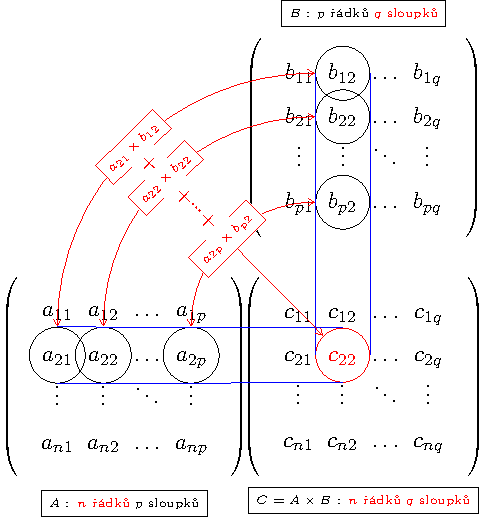
\includegraphics[width=0.45\linewidth]{mai_fig023a}}               &
        \subfloat[2. krok]{\label{LA:fig_LA001b}
          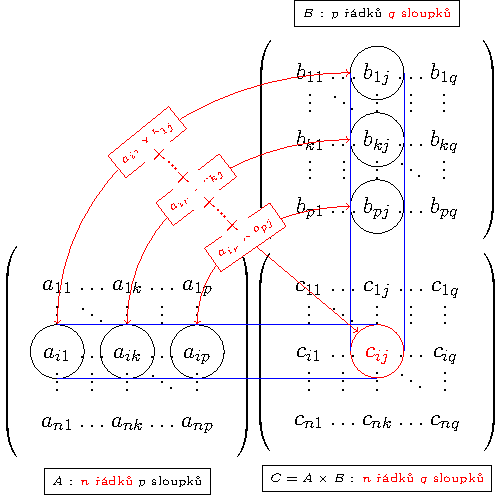
\includegraphics[width=0.45\linewidth]{mai_fig023b}} 
      \end{tabular}
      \caption{Postup při maticovém násobení}
    \end{figure}
  

      
      \begin{definition}\label{rovnost_matic}
       (Rovnost matic):  Matice \(\matr{A} = \left(a_{ij}\right)\) je rovna matici \(\matr{B}=
       \left(b_{kl}\right)\), jsou-li matice stejného typu a stejnolehlé prvky se sobě
       \textbf{rovnají}, tj. \(\matr{A} \in \mathbb{R}_{m,n}, \matr{B}\in\mathbb{R}_{m,n}, 
       a_{ij} = b_{ij}, \forall i\in\lbrace1,2,\ldots,m\rbrace, \forall j\in\lbrace1,2, \ldots 
       ,n\rbrace\).
      \end{definition}
      
%--------------------------------------------------------------------------------------------------
  \section{Počítání s vektory}\label{mai:IchapIIsecIV}
    \textbf{Vektory} budeme nazývat matice typu \(1/n\) a značit je
    \begin{equation*}
      \vec{u} = (u_1, u_2, \ldots, u_n).
    \end{equation*}
    Takže počítat s nimi již umíme! (V zápisu složek vektoru je vynechán řádkový index. V případě 
    matice s jedním řádkem, takzvané \emph{řádkové matice}, je totiž zbytečný.) Číslům \(u_1\) až 
    \(u_n\) budeme pro tuto chvíli říkat \emph{složky vektoru} \(\vec{u}\). Za chvíli tento pojem 
    ještě upřesníme. Celou řadu pojmů, s nimiž jsme se seznámili při počítání s maticemi, můžeme 
    pro vektory přímo použít. Namísto značení \(\mathcal{M} (1/n)\) budeme pro prostor vektorů 
    používat symbol \((\mathbb{R}^n)\) nebo \(\mathbb{C}^n\) (obvyklý symbol pro množinu 
    uspořádaných \(n\)-tic reálných nebo komplexních čísel).
    
    \subsection{Součiny vektorů}
      Kromě základních operací s vektory, tj. sčítání vektorů a násobení vektoru skalárem, se 
      často používají další operace, které obohacují \emph{strukturu vektorového prostoru}. 
      Zůstaneme u vektorů v trojrozměrném prostoru \(\mathbb{R}^3\) a definujeme si skalární, 
      vektorový a smíšený součin vektorů. Skalární součin vektorů definujeme prostřednictvím 
      geometrické definice jako zobrazení, které uspořádané dvojici vektorů (volných vektorů nebo 
      jejich libovolných umístění) přiřazuje reálný číslo podle předpisu
      \begin{equation}\label{mai:eq038}
        \vec{u}\vec{v} = \abs{\vec{u}}\cdot\abs{\vec{v}}\cos\varphi,
      \end{equation}
      kde \(\varphi = \sphericalangle(\vec{u},\vec{v})\) je velikost minimálního z obou úhlů mezi 
      vektory\(\vec{u},\vec{v}\).

    %---------------------------------------------------------------
    % !TeX spellcheck = cs_CZ
% \wikitextrule
\begin{mdframed}[style=mdexam]
  \begin{example}\label{mai:exam034}
    Vypočteme z definice \ref{mai:eq038} skalární součiny vektorů ortonormální báze \(\vec{e_1}\), 
    \(\vec{e_2}\) a \(\vec{e_3}\), spjaté s kartézskou soustavou souřadnic. Připomeňme, že tyto 
    vektory jsou jednotkové a navzájem kolmé.
    \begin{itemize}
      \item pro \(i\neq j\) \(\vec{e_i}\vec{e_j}=0\), 
                \(\sphericalangle\vec{e_i}\vec{e_j} =\dfrac{\pi}{2}\), vektory jsou kolmé,
      \item pro \(i = j\) \(\vec{e_i}\vec{e_j}=0\), 
                \(\sphericalangle\vec{e_i}\vec{e_j} =0, \abs{\vec{e_i}}=1\), vektory jsou 
                jednotkové.
    \end{itemize}

    Pro skalární součiny vektorů ortonormální báze použijeme zkrácené značení
    \begin{equation}\label{mai:eq085}
      \vec{e_i}\vec{e_j} = \delta_{ij},
    \end{equation}
    kde \(\delta_{ij}\) nabývá hodnoty \num{1} pro \(i = j\) a hodnoty \num{0} pro \(i \neq j\). 
    Nazývá se \textbf{Kroneckerovo delta} \cite[s.~40]{Musilova2009MA1}.
  \end{example}
\end{mdframed}
    %---------------------------------------------------------------
    
    Shrneme nyní vlastnosti skalárního součinu. Dokázat bychom je mohli, i když by to mohlo být i 
    velmi pracné, užitím znalostí z goniometrie. Zkuste to alespoň pro jednu z nich! Třeba se    
    vám podaří zvolit si tu nejjednodušší.

%} % tikzset
%---------------------------------------------------------------------------------------------------
\printbibliography[title={Seznam literatury}, heading=subbibliography]
\addcontentsline{toc}{section}{Seznam literatury}